\chapter{Felhasználói dokumentáció}

\section{A megoldott feladat}

A program lehetővé teszi a prímek néhány statisztikájának ábrázolását grafikonon,
és összevetését elméleti becsült értékekkel, valamint néhány különböző szita-algoritmus
futási idejének megmérését, és grafikus megjelenítését.
A programmal egyéb forrásból származó minták megjelenítése is lehetséges.

A prímszámok statisztikáinak előállításához a programhoz tartozik egy optimalizált
szita-implementáció, amivel $2^{64}$-ig lehet szitálni, és az eredményt rögzíteni.
Az elmentett prímlistákat a program összesíti több statisztika szerint, és a megjelenítést az összesítések alapján végzi el.

A különböző szita-algoritmusok futási idejének összehasonlításához a program tartalmazza
Atkin\cite{atkin} szitájának egy implementációját, és Eratoszthenész szitájának néhány variációját. Ezek a sziták a prímek statisztikáinak előállításában nem vesznek részt.

\section{A szoftver komponensei}

A program két elkülönülő részből áll.
A prímszámok statisztikáinak előállításához először szükséges a prímek listájának előállítása.
Ehhez egy optimalizált, gyors szita C nyelven készült el.
A könnyebb implementálhatóság miatt ez is két külön program, a kis számokat szitáló \texttt{init}, és a nagyobb számokkal dolgozó \texttt{generator}.
Az \texttt{init} és a \texttt{generator} program a működési elvében hasonló.

A program többi része Java nyelven van megírva, ez a \texttt{gui} nevű program.
Ez összesíti a prímek listáját, tartalmazza a futási idők összehasonlításához írt szitákat, és jeleníti meg a prímek statisztikáit, és a futási idők mintáit.

Ez a három program az ``adatbázis könyvtárba'' mentett bináris fájlokon keresztül kommunikál.
Ide kerülnek az elkészült szitatáblák, és a prímek statisztikái.

\begin{figure}[H]
\centering
\caption{A program komponensei és adatáramlás diagramja}
\begin{tikzpicture}[framed]
\draw (0, 0) node[rectangle,draw](db) {Adatbázis};

\draw (-1, 1) node[rectangle,rounded corners,,draw](init) {\texttt{init}};
\draw (1, 1) node[rectangle,rounded corners,,draw](generator) {\texttt{generator}};
\draw (4, 1) node[rectangle,rounded corners,,draw](aggregate) {Összesítés};
\draw (4, 0) node[rectangle,draw](info) {Info};

\draw (-4, 1) node[rectangle,rounded corners,draw](check-segment) {Szegmens ellenőrzése};
\draw (-4, 0) node[rectangle,rounded corners,,draw](reference-sieve) {Referencia szita};
\draw (-4, -1) node[rectangle,rounded corners,,draw](check-sieve) {Szita ellenőrzése};
\draw (0, -1) node[rectangle,rounded corners,,draw](sieves) {Sziták};

\draw (4, -1) node[rectangle,draw](view) {Megjelenítés};
\draw (4, -2) node[rectangle,rounded corners,,draw](approximate) {Minta közelítése};

\draw[<->, thick] (db) -- (aggregate);
\draw[->, thick] (db) -- (check-segment);
\draw[<->, thick] (db) -- (generator);
\draw[->, thick] (db) -- (info);
\draw[->, thick] (db) -- (reference-sieve);
\draw[->, thick] (db) -- (sieves);
\draw[->, thick] (db) -- (view);
\draw[->, thick] (init) -- (db);
\draw[->, thick] (reference-sieve) -- (check-segment);
\draw[->, thick] (reference-sieve) -- (check-sieve);
\draw[->, thick] (sieves) -- (check-sieve);
\draw[->, thick] (sieves) -- (view);
\draw[<->, thick] (view) -- (approximate);

\draw[dashed, rounded corners] (-6.2, 0) -- (-6.2, 1.5) -- (-1.7, 1.5) -- (-1.7, -0.5) -- (2.7, -0.5) -- (2.7, 1.5) -- (5.8, 1.5) -- (5.8, -2.5) -- (-6.2, -2.5) -- (-6.2, 0);
\draw (-5.7, -2.2) node[]{\texttt{gui}};
\draw[dashed, rounded corners] (-6.2, -1.8) -- (-5.1, -1.8) -- (-5.1, -2.5);
\end{tikzpicture}
\end{figure}

A programok több prímszitát tartalmaznak.
A prímsziták számok egy intervallumáról döntik el, hogy melyik szám prím, és melyik összetett.
A legtöbb implementált szita Eratoszthenész szitájának változata.
Eratoszthenész szitája az egész számok egy adott $[2, n]$ intervallumába eső számokról dönti el, hogy melyik prím.
Ezt a $pq$ szorzatra bontható számok megjelölésével teszi, ahol a $p<n$ prím, és $1<q\in\mathbb{N}$.
Az algoritmus sorban veszi a számokat a listában kettőtől.
Ha egy addig még meg nem jelölt számot talál, akkor az prím, és a listában megjelöli annak többszöröseit, de a prímet nem.
Az algoritmus futása után a meg nem jelölt számok a prímek.

\begin{algorithmic}[1]
\State $n$: \text{a szitálás felső határa}
\State \text{a számok legyenek nem megjelölve, 2-től $n$-ig}
\For{$i \gets 2$, $i \le n$, $i \gets i+1$}
	\If{$i$ nincs megjelölve}
		\For{$j \gets i^2$, $j \le n$, $j \gets j+i$}
			\State \text{legyen $j$ megjelölve}
		\EndFor
	\EndIf
\EndFor
\end{algorithmic}

Ennek az egyszerű algoritmusnak a egyik hátránya, hogy $n$-ig szitálva $n-1$ bit memóriára van szüksége, ez a bitvektor a szitatábla.
Erre megoldás a szegmentált szitálás, ahol egy rövidebb, nem feltétlenül 2-től kezdődő intervallumban szitálnak.
Ehhez szükség van a prímek listájára, legalább az intervallum végének négyzetgyökéig.

A legegyszerűbb szegmentált szita egy szegmens szitáláshoz minden prímet sorban vesz az intervallum végének négyzetgyökéig, osztással meghatározza, hogy melyik a legkisebb többszöröse a szegmensben, és ha van ilyen szám, akkor onnantól összeadással szitál a prímmel a szegmens végéig, ahogy Eratoszthenész szitája is teszi.

Több, egymás utáni szegmens szitálásával az osztás költsége több szegmensre szétosztható, ha a szita a minden prímről minden szegmens szitálása után megjegyzi, hogy melyik számot szitálna, ami már nagyobb, mint a szegmens vége.
A következő szegmens feldolgozásakor a prímmel innen lehet folytatni a szitálást.
A módszer hátránya, hogy ehhez el kell tárolni ezeket a prím-pozíció párokat, ennek tárigénye nagyságrendileg $\mathcal{O}(\sqrt{n})$ bit, ha legnagyobb szitált szám $n$.
A hatékony eratoszthenészi sziták ennek a prím-pozíció listának csak azon elemeit veszik figyelembe egy szegmens szitálásakor, amik ténylegesen szitálnak is a szegmensben.

\subsection{Init és generator program}

A prímszámok listájának generátora C nyelven készült el.
A program csak parancssorból futtatható, és a sztenderd könyvtári függvényekből
is csak néhányat használ a memóriájában előállított eredmények fájlba írásához.
A C nyelv választását a hatékony végrehajtás és memóriafelhasználás, valamint a hordozhatóság indokolja. A generátor elkülönítését a \texttt{gui} programtól az automatizálhatóság indokolja.

A prímlisták generátora Eratoszthenész szitájának szegmentált változata,
a szitatábla egy $2^{30}$ hosszú darabját szitálja ki minden iterációban.
Ez a generátor önmaga is két részből áll.
Az egyszerűbb implementációjú \texttt{init} a prímek listáját $2^{32}$-ig állítja elő.
Ezekre a prímekre nem csak a statisztikák előállítása miatt van szükséges, hanem a \texttt{generator}, és a \texttt{gui} program szitái is használják, amikor a szitálás intervalluma 3-nál nagyobb számtól kezdődik.

A gyorsabb, de összetettebb \texttt{generator} $2^{32}$-től $2^{64}-2^{34}$-ig szitál,
és a futásához szükséges a prímek listája $2^{32}$-ig.
A szitatáblát a memóriában a gyorsítótár hatékonyabb a kihasználásához kisebb
részszegmensekre osztja, és a prímeket a nagyságuk és a következő szitálási pozíciójuk szerint csoportosítja.
Továbbá nagyobb prímeknek csak harminccal relatív prím többszöröseit veszi figyelembe.

\subsection{Gui}

A program többi része a Java környezethez készült, ez a \texttt{gui} program.
Ez végzi a \texttt{generator} által előállított szegmensfájlok összesítését, és az elkészült statisztikák megjelenítését.

A \texttt{generator} a szegmensfájlokat az adatbázis könyvtáron keresztül adja át a \texttt{gui} programnak, és az összesítések is ebbe a könyvtárba kerülnek.
A szegmensfájlokra az ellenőrzés és összesítés után már nincs szükség, ezek eltávolíthatóak.
Az adatbázisában hosszabb távon egyedül a prímek szegmensenkénti statisztikáit kell tárolni.
A \texttt{gui} program a statisztikákat csak sorban dolgozza fel, és a statisztikák összmérete sem indokol egy egyszerű bináris fájlnál bonyolultabb megoldást.

\subsubsection{Megjelenítés}

A \texttt{gui} képes egyváltozós mintákat megjeleníteni Descartes-féle koordináta rendszerben.
A minták értékkészlete a természetes számok, az értelmezési tartomány a valós számok.
Ezek a minták a szitálással gyűjtött statisztikákból származhatnak, vagy külső forrásból is betölthető minta az $(x, y)$ párok felsorolásával.

Lehetséges a mintákat alapfüggvények lineáris kombinációjával közelíteni.
Az alapfüggvényeket beépített függvényekből lehet kiválasztani, vagy JavaScript nyelven is meg lehet adni.
A közelítő függvény és a minta grafikonját a program együtt jeleníti meg, ezzel a hibát nem csak numerikusan adja meg a program, hanem szemlélteti is.

\subsubsection{Sziták}

A \texttt{gui} program tartalmaz több prímszita implementációt is. Ezeknek az algoritmikus bonyolultsága különböző, de a futási idejük összehasonlíthatóságához a közös részek közös implementációt kaptak, és az eltérő részek hasonló szinten optimalizáltak.
A sziták helyességének ellenőrzéséhez a sziták eredménye egymással összehasonlítható.

Elkészült Eratoszthenész szitájának több variációja, mindegyik szegmentáltan működik, a különbség a prímek listájának kezelésében van.
A legegyszerűbben implementált eratoszthenészi szita a prímek listáját minden szegmensben végig bejárja.
A prioritásos soron alapuló sziták a prímeket részlegesen rendezik az alapján, hogy hány szegmensnyire van az éppen szitált szegmenstől a prím következő többszöröse.
Ilyen a bináris kupacot, és az edénysort használó szita.

A Cache Optimalizált Lineáris Szita\cite{cols} a prímeket teljesen rendezi az alapján, hogy legközelebb melyik szegmensben fognak szitálni, és a prímek nagyság szerinti csoportosításával a rendezés fenntartásához az elemek memóriabeli mozgatását is kerüli.

Atkin szitája\cite{atkin} az előbbi algoritmusoktól jelentősen eltér, a prímek többszörösei
helyett $n=ax^2+by^2$ egyenlet megoldásait keresi egy $n$ szám vizsgálatához, $x$ és $y$ pozitív egészek befutásával, $a$ és $b$ egész konstansok.
A pontos kvadratikus formát, és $x$ és $y$ lehetséges értékeit Atkin az egészek algebrai bővítésével határozza meg, $n \in 4\mathbb{Z}+1$ esetén a Gauss-egészek, $n \in 6\mathbb{Z}+1$ esetén az Eisenstein-egészek, és $n \in 12\mathbb{Z}+11$ esetén a $\mathbb{Z}[\sqrt{3}]$ segítségével.

A sziták között kapott helyet a próbaosztás, és a Miller–Rabin pszeudoprím teszt\cite{miller} is, de ezek a lassúságuk miatt csak igen rövid tartományokon használhatóak.
A próbaosztás egy faktorizációs eljárás, ami egyetlen számot nem-triviális szorzatra próbál bontani.
Az (erős) pszeudoprím teszt egy prímteszt, egyetlen számról próbálja eldönteni, hogy az prím-e.
A prímteszteket általában több nagyságrenddel nagyobb számokra alkalmazzák, mint a szitákat, és teljes módszer helyett sokszor megelégednek egy valószínűségi válasszal.

\section{A program telepítése és futtatása}

A program futtatásához Windows vagy Linux operációs rendszer szükséges, legalább 4GB szabad memóriával.
A Java program futtatásához JRE8 szükséges, a fordításához JDK8.
A C program fordításához C99 szabványú fordítóprogram kell.
A program fejlesztése és tesztelése OpenJDK8-cal és GCC 7.3-mal történt Linux operációs rendszeren.

A teljes program letölthető a \url{https://github.com/zooflavor/lazysieve} címről, vagy megtalálható a CD mellékleten.
A CD mellékleten található tarball a Java programot lefordítva is tartalmazza, kicsomagolás után azonnal futtatható.
A C programot a \texttt{generator} könyvtárban található \texttt{Makefile} segítségével lehet lefordítani:
\begin{lstlisting}[language=bash]
generator$ make clean build
\end{lstlisting}

A Java program a NetBeans 8-as verziójával készült,
parancssorból a project ant fájlának segítségével lehet újrafordítani:
\begin{lstlisting}[language=bash]
gui$ ant clean jar
\end{lstlisting}

A program futtatásához több előkészített szkript is rendelkezésre áll, ezeket mind a \texttt{scripts} könyvtárból lehet indítani.
Az előző két fordítást egyben is el lehet végezni a \texttt{recompile} szkripttel:
\begin{lstlisting}[language=bash]
scripts$ ./recompile
\end{lstlisting}

\section{Prímek keresése}

A prímek keresését két program végzi, az \texttt{init} program $2^{32}$-ig keresi meg és tárolja el a prímeket, a \texttt{generator} $2^{32}$-től $2^{64}-2^{34}$-ig.
Az \texttt{init} készítette szitattáblák a \texttt{generator} futásához szükségesek.

Mindkét program a számokat $2^{30}$ hosszú táblánkként szitálja, minden tábla első száma $k \cdot 2^{30}+1$ alakú.
A szitatáblában csak a páratlan számok vannak nyilvántartva.
A szitatáblákat a programok a fájlrendszerben bitvektorként tárolják, egy tábla kb. $64$Mb.

Az első négymilliárd szám szitálása a következőképpen indítható el:

\begin{lstlisting}[language=bash]
generator$ ./init.bin ../db
szegmens 0 - kezdet             1 - felkészülés 159 906 063 ns - szitálás 1 122 878 403 ns
szegmens 1 - kezdet 1 073 741 825 - felkészülés   2 353 698 ns - szitálás 1 171 101 336 ns
szegmens 2 - kezdet 2 147 483 649 - felkészülés   2 344 515 ns - szitálás 1 188 330 478 ns
szegmens 3 - kezdet 3 221 225 473 - felkészülés   2 391 660 ns - szitálás 1 199 900 603 ns
\end{lstlisting}
Ennek eredmény 4 bitvektort tartalmazó bináris fájl, amit a \texttt{db} mappába ment.

A \texttt{generator} program minden olyan paraméterét, ami szám, meg lehet adni decimálisan, és hexadecimálisan is \texttt{0x} előtaggal.
A számok hexadecimális megadásának lehetősége a \text{gui} programot hívó szkripteknél is megvan.

A \texttt{generator} programot többféleképpen is lehet indítani.
Mindegyik esetben két paramétert kell megadni az indításhoz, a számot, ahol szitálást kezdje, és a szegmensek számát, amit ebben a futásban végig kell szitálni.
A szegmensek számát kétféleképpen lehet szabályozni.
Az egyik lehetőség fix számú szegmens megadása.

\begin{lstlisting}[language=bash]
generator$ ./generator.bin ../db start 0x100000001 segments 3
szegmens kezdet: 4 294 967 297
szegmensek száma: 3
kis szegmensek mérete: 22
elágazások bitjei: 8
felkészülés 1/4
felkészülés 2/4
felkészülés 3/4
felkészülés 4/4
felkészülés vége
szegmens 4 - kezdet 4 294 967 297 - felkészülés 8 162 031 487 ns - szitálás 729 914 370 ns
szegmens 5 - kezdet 5 368 709 121 - felkészülés           418 ns - szitálás 736 412 117 ns
szegmens 6 - kezdet 6 442 450 945 - felkészülés           385 ns - szitálás 750 022 409 ns
összes szitálás 2 216 348 896 ns
\end{lstlisting}

A másik mód a háttértáron fenntartandó szabad hely átadása, ezt bájtokban kell megadni.
Ekkor minden szegmens szitálása előtt megvizsgálja, hogy van-e még annyi szabad hely az adatbáziskönyvtárban, mint amennyi meg van adva, ha igen, akkor szitálja a szegmenst,
és lép a következőre, és ha nincs már elég szabad hely, akkor a program leáll.

\begin{lstlisting}[language=bash]
generator$ ./generator.bin ../db start 0x100000001 reserve-space 1000000000
szegmens kezdet: 4 294 967 297
fenntartandó hely: 1 000 000 000 byte 
kis szegmensek mérete: 22
elágazások bitjei: 8
felkészülés 1/4
felkészülés 2/4
felkészülés 3/4
felkészülés 4/4
felkészülés vége
szegmens 4 - kezdet 4 294 967 297 - felkészülés 8 162 031 487 ns - szitálás 729 914 370 ns
szegmens 5 - kezdet 5 368 709 121 - felkészülés           418 ns - szitálás 736 412 117 ns
szegmens 6 - kezdet 6 442 450 945 - felkészülés           385 ns - szitálás 750 022 409 ns
összes szitálás 2 216 348 896 ns
\end{lstlisting}

Mindkét program kimenetében a ''start'' a szegmens kezdőszáma, a ''szegmens'' az indexe,
$start=szegmens \cdot 2^{30}+1$, a ''felkészülés'' a szita inicializálási ideje a szitálás előtt,
és a 'szitálás' a szegmens szitálásának ideje.
Ezek az információk az elmentett szegmensfájlokból is kiolvashatóak.

\section{Az adatbázis karbantartása}

A \texttt{init} és \texttt{generator} programok az elkészült szitatáblákat az adatbáziskönyvtárba mentik.
Minden szitatábla külön ''szegmensfájlba'' kerül.
A szegmensfájlok neve \texttt{primes.}-szal kezdődik, és pontosan 16 hexadecimális karakter követi.
Ez a 16 jegyű szám a szegmens első száma.
A fájl a páratlan számok bitvektora mellett tartalmazza a szegmens szitálásának megkezdésére, és a szitálására fordított időt, valamint ellenőrzésképpen a szegmens kezdőszámát is.

A szitatáblák mellett az adatbázis tartalmazhatja szegmensek összesített statisztikáit is, \texttt{aggregates} néven.
Ez a fájl az eddig összesített szegmensekről a következő információkat tartja nyilván, minden szegmensről külön-külön:
\begin{itemize}
\item a szegmens kezdőszáma
\item a szegmens szitálására való felkészülés idejét
\item a szegmens szitálásának idejét
\item az összesítésre fordított időt
\item a szegmensfájl utolsó módosítási idejét
\item a szegmensbe eső legkisebb, és legnagyobb prímet
\item a szegmensbe eső $4\mathbb{Z}+1$, $4\mathbb{Z}+3$, $6\mathbb{Z}+1$ és $12\mathbb{Z}+11$ alakú prímek számát külön-külön
\item a szegmensben előforduló prímhézagok első előfordulásának helyét, és az előfordulások számát.
\end{itemize}

Példaként ha a szegmensek mérete 16 szám lenne, és 17-től szitálnánk egy szegmensnyit, akkor a szegmensfájl leírná, hogy a prímek a 17, 19, 23, 29, 31, és az összetett számok a 15, 21, 25, 27.
A szegmens összesítése azt tartalmazná, hogy
\begin{itemize}
\item a szegmens 17-tel kezdődik
\item a legkisebb prím 17, a legnagyobb 31
\item a szegmensben
\begin{itemize}
\item 2db $4\mathbb{Z}+1$
\item 3db $4\mathbb{Z}+3$
\item 2db $6\mathbb{Z}+1$
\item 1db $12\mathbb{Z}+11$ alakú prím van
\end{itemize}
\item a szegmensben előforduló prímhézagok
\begin{itemize}
\item a 2 (ikerprímek) kétszer fordul elő, először 17-nél
\item a 4 egyszer fordul elő, először 19-nél
\item a 6 egyszer fordul elő, először 23-nál.
\end{itemize}
\end{itemize}

\subsection{Adatbázis műveletei}

Az adatbázison három művelet végezhető:
\begin{itemize}

\item Le lehet kérni
\begin{itemize}
\item a szegmensfájlok számát
\item az első és utolsó szegmensfájlt
\item az legkisebb hiányzó szegmensfájlt
\item a szegmensstatisztikák számát
\item az első és utolsó szegmensstatisztikát
\item az legkisebb hiányzó szegmensstatisztikát
\item az összesítést igénylő új szegmensfájlok számát.
\end{itemize}

\item Összesíteni lehet az új szegmensfájlokat.

\item Össze lehet fésülni két összesítőfájlt.

\end{itemize}

Mindhárom művelet elvégezhető a grafikus felületen, és automatizáláshoz parancssorból is.
A grafikus felületet a \texttt{gui} szkripttel lehet indítani, a parancssorból a \texttt{database} szkript segítségével lehet elérni a műveleteket.

A \texttt{gui} programnak az adatbázis könyvtár helye ugyanúgy paraméter, ahogy az \texttt{init}-nek és a \texttt{generator}-nak. Ezt a könyvtárat a \texttt{gui} és a \texttt{database} szkriptek beégetve tartalmazzák, ezt nem kell külön megadni.
A beégetett könyvtár a \texttt{../db}.
Szükség esetén ez a könyvtár a szkriptek egyszerű módosításával megváltoztatható, a \texttt{DB} változónak adott érték átírásával.

\subsection{Adatbázis információk}

A adatbázis információkat a grafikus felületen a ''DB info'' gomb megnyomásával lehet
lekérdezni, parancssorból a \texttt{database info} kiadásával.

\begin{lstlisting}[language=bash]
scripts$ ./database info
100.0%
szegmensfájlok: szegmensek száma: 7
szegmensfájlok: első szegmens kezdete: 1
szegmensfájlok: utolsó szegmens kezdete: 6,442,450,945
szegmensfájlok: első hiányzó szegmens kezdete: 7,516,192,769
szegmensfájlok: hiányzó szegmensek száma: 18,446,744,073,709,551,593

összesítések: szegmensek száma: 62,881
összesítések: első szegmens kezdete: 1
összesítések: utolsó szegmens kezdete: 67,516,885,893,121
összesítések: első hiányzó szegmens kezdete: 67,517,959,634,945
összesítések: hiányzó szegmensek száma: 18,446,744,073,709,488,719

új szegmensfájlok: 7

scripts$ ./database info crunch 1024
100.0%                     
szegmensfájlok: szegmensek száma: 4
szegmensfájlok: első szegmens kezdete: 1
szegmensfájlok: utolsó szegmens kezdete: 3,221,225,473
szegmensfájlok: első hiányzó szegmens kezdete: 4,294,967,297
szegmensfájlok: hiányzó szegmensek száma: 18,446,744,073,709,551,596

összesítések: szegmensek száma: 140,292
összesítések: első szegmens kezdete: 1
összesítések: utolsó szegmens kezdete: 150,636,314,230,785
összesítések: első hiányzó szegmens kezdete: 150,637,387,972,609
összesítések: hiányzó szegmensek száma: 18,446,744,073,709,411,308

crunch: ../generator/generator.bin ../db start 0x890100000001 segments 0x400
\end{lstlisting}

A \texttt{crunch} paraméter és a szitálni kívánt szegmensek számának megadásával az utolsó sorban
a következő futtatásra ajánlott parancsot is megjeleníti a program.
Ezeknek a parancsoknak a követésével a teljes szitálható tartományt fel lehetne dolgozni.
A \texttt{crunch-numbers} szkript ezt a feladatot kísérli meg elvégezni.

A \texttt{database info} megjeleníti az új szegmensfájlok számát is, ezek azok, amikhez vagy nem tartozik összesített adat, vagy tartozik, de az régebbi szegmensfájl alapján készült, mint ami éppen az adatbáziskönyvtárban található.

\begin{figure}[h]
\caption{Adatbázis információk}
\centering
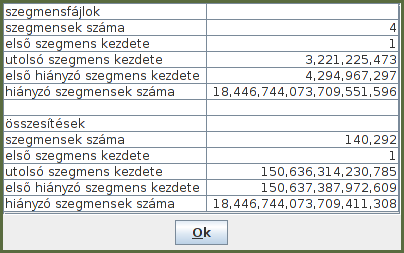
\includegraphics[scale=1]{info.png}
\end{figure}

\subsection{Szegmensek összesítése}

Az adatbázis könyvtárban található új szegmensfájlokat a ''DB összesítés'' gomb megnyomásával, vagy a \texttt{database reaggregate} paranccsal lehet összesíteni.
Minden olyan szegmensfájlról új összesítés készül, amihez még nem tartozott összesítés, vagy a szegmensfájl újabb, mint ami alapján a már meglévő összesítés készült.
Az adatbázisban már meglévő, többi szegmenshez tartozó statisztika nem vész el.

\begin{lstlisting}[language=bash]
scripts$ ./database reaggregate
100.0%
\end{lstlisting}

\subsection{Összesítőfájlok összefésülése}

Lehetőség van egy másik adatbázisból statisztikák átvételére is.
Erre több gépen párhuzamosan szitálva lehet szükség.
Az összefésülést a grafikus felületen a ''DB import'' megnyomása után egy file kiválasztásával lehet indítani.
Parancssorból a \texttt{dabatase import aggregates} \textit{fájlnév} parancs kiadásával.
A megadott fájlból azokat a szegmenseket veszi át a program, amik vagy nincsenek még meg az adatbázisban, vagy megvannak, de az importált statisztikák utolsó módosítási ideje nagyobb az adatbázisban lévőnél.

\begin{lstlisting}[language=bash]
scripts$ ./database import aggregates /valahol/egy/masik/aggregates
100.0%
\end{lstlisting}

\section{Szitatáblák ellenőrzése}

A \texttt{generator} program teszteléséhez a grafikus program képes a szegmensfájlok ellenőrzésére.
Ehhez a \texttt{gui} újra előállítja az ellenőrzött szegmensfájlokat, és azokat összeveti.
Az ellenőrzőszegmensek előállításához az egyszerű szegmentált eratoszthenészi szitát, vagy ez erős pszeudoprím tesztet lehet választani.

A pszeudoprím teszt a szegmens minden számáról egyesével dönti el, hogy az prím-e.
A pszeudoprím teszt rendkívül lassú, a célja, hogy Eratoszthenész szitájához képest egy alapvetően más módszer is rendelkezésre álljon az ellenőrzéshez.

A grafikus felületen a ''Szegmensfájlok ellenőrzése'' gomb megnyomása után lehet kiválasztani a szitálni kívánt szegmenseket, és a referencia előállításának módszerét, majd az ''Ellenőrzés'' gombbal lehet megkezdeni a tényleges folyamatot.

Az ellenőrzést parancssorból is lehet futtatni a \texttt{check-segments} szkripttel.
A szkript első paraméterében a referencia módszerét várja, ami lehet \texttt{sieve}, vagy \texttt{test}, a paraméterek maradéka az ellenőrizendő szegmensek kezdőszáma kell legyen.
Ha egy kezdőszám sincs megadva, akkor a program az adatbázis könyvtárban található összes szegmensfájlt ellenőrzi.

\begin{lstlisting}[language=bash]
scripts$ ./check-segments sieve
100.0%: A szegmensek helyesek.             

scripts$ ./check-segments sieve 0x1 0xc0000001
100.0%: A szegmensek helyesek.             

scripts$ ./check-segments test 0x1
100.0%: A szegmensek helyesek.             

\end{lstlisting}

Az ellenőrzőszegmens szitával történő előállításához szükséges, hogy az \texttt{init} program által előállított négy darab szegmensfájlt tartalmazza az adatbáziskönyvtár.
Az $1$-től kezdődő szegmens kivételével az ellenőrző szegmens előállításához a szita az inicializálásához a prímszámokat innen olvassa fel.

\section{Sziták ellenőrzése}
\label{sec:szitak-ellenorzese}
%%% EMIL: az előző fejezet szatatáblák ellenőrzése volt... ami nagyon hasonlít ehhez a fejezethez... mi a különbség?
%%% P: 1-2 olvasáskörig megfontolom, hogy a "sziták"-at át lehetne nevezve, "a versenyló sziták"- szerű kifejezésre


A sziták futási idejének összehasonlításához írt szitákat is lehet ellenőrizni, az általuk előállított szitatáblák ellenőrzésével.
Az összehasonlításhoz a szegmensek ellenőrzésénél használt egyszerű szegmentált szita a referencia.

A program grafikus felületén a ''Sziták ellenőrzése'' lehetőséget választva ki kell választani az ellenőrizendő szitát, és az ellenőrizni kívánt intervallum kezdő és végző számát.
A folyamat az ''Ellenőrzés'' gomb megnyomásával indítható.

Parancssorból is ellenőrizhetőek a sziták a \texttt{check-sieve} szkripttel.
A szkript 3 paramétere a szita neve, és az intervallum kezdő-, és végszáma.
Az ellenőrizhető sziták nevei:
\begin{itemize}
\item \texttt{atkin}: Atkin szitája\cite{atkin}
\item \texttt{cols}: Cache Optimalizált Lineáris Szita\cite{cols}
\item \texttt{eratosthenes-segmented}: Eratoszthenész szitájának szegmentált változata
\item \texttt{bin-heap} és \texttt{bin-heap-inplace}: Eratoszthenész szitája bináris kupaccal,
	a \texttt{bin-heap-inplace} a kupac javítását helyben végzi
\item \texttt{buckets}, \texttt{buckets-}$n$, \texttt{buckets-simple}: Eratoszthenész szitája, edénysorral
	A \texttt{buckets-simple} nem szegmentált, a \texttt{buckets}, és a \texttt{buckets-}$n$ szegmentált.
	A \texttt{buckets-}$n$-ben az $n$ helyére 1-től 8-ig a számrendszer bitjeit lehet megadni,
	pl. \texttt{buckets-3} 8-as számrendszerben számol
\item \texttt{trial-division}: próbaosztás
\end{itemize}

A \pageref{sec:szitak} oldalon található ''Sziták'' szakaszban található ezeknek a szitáknak a részletesebb leírása.

A sziták nevei listázhatóak a \texttt{list-sieves} szkripttel, a \texttt{describe-sieves} szkript rövid leírást is ad.

\begin{lstlisting}[language=bash]
scripts$ ./check-sieve buckets-3 3000000000001 3010000000001
100.0%: A szita helyes.
\end{lstlisting}

Ha a kezdőszám nagyobb, mint 1, az ellenőrzéshez ilyenkor is szükséges, hogy a négy darab kezdő szegmensfájlt tartalmazza az adatbáziskönyvtár.

\begin{figure}[h]
\caption{Szita ellenőrzése}
\centering
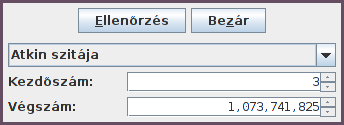
\includegraphics[scale=1]{check-sieve.png}
\end{figure}

\section{Minta megjelenítése}

A \texttt{gui} program a grafikus felületén képes mintákat Descartes-féle koordináta rendszerben ábrázolni, a mintákat függvényekkel közelíteni, és ezeket a függvényeket a mintával együtt ábrázolni.
A program a közelítések négyzetes hibáját is kiszámítja a mintához képest.
A program egyváltozós, egyértékű mintákat kezel, azok között is a természetes számokhoz valós számokat rendelőket.
A minta akár külső forrásból is származhat.

A grafikonábrázoló részt a \texttt{gui-graph} szkripttel lehet indítani. A \texttt{gui} szkripttel indítva, majd a ''Grafikon'' gomb megnyomásával is meg lehet nyitni ezt az ablakot.

Az ablak bal oldalán jelennek meg a betöltött minták és közelítő függvények grafikonjai.
Minta és függvény hozzáadása után a grafikon megjelenített részét a program úgy választja meg, hogy minden minta összes pontja ebbe a nézetbe essen.
A nézet a grafikon feletti gombokkal, vagy egérrel mozgatható, nagyítható, vagy kicsinyíthető.
Az ''Auto.nézet'' gombbal a nézet a minták teljes terjedelmére visszaállítható.

Az ablak jobb oldala a betöltött minták kezelésére szolgál.
A felső harmada az összes betöltött mintát mutatja.
Az ablak jobb oldalának alsó két harmadában az itt kiválasztott minta részletei látszódnak.

\begin{figure}[h]
\caption{Minta megjelenítése}
\centering
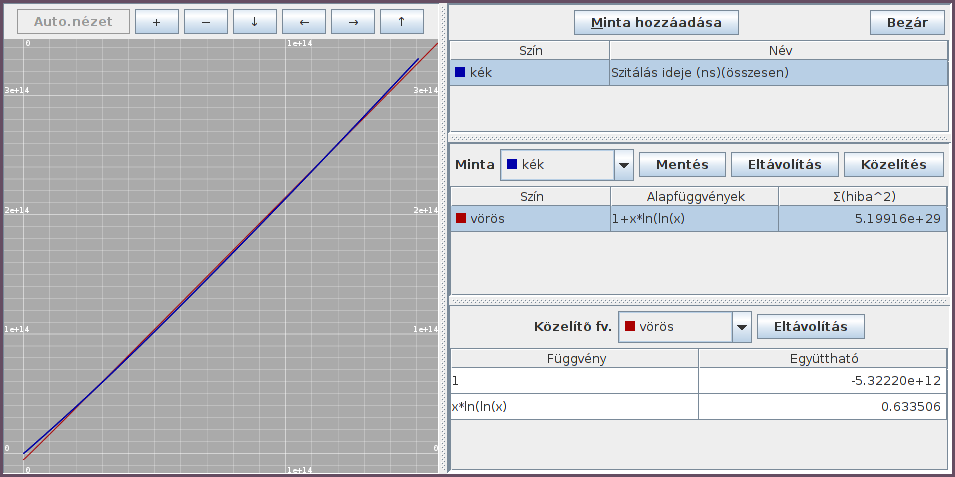
\includegraphics[scale=0.5]{graph.png}
\end{figure}

\subsection{Minta hozzáadása}

A ''Minta hozzáadásánál'' három adatforrásból lehet választani.
A ''Fájl betöltésével'' CSV fájl olvasható be. A fájl formátuma megengedő, az első oszlopot $x$, a második oszlopot $y$ értékeknek próbálja értelmezni, a fel nem ismert sorokat eldobja.
Ha az első sor első oszlopában \texttt{BARS} szerepel, akkor a program a mintát vonaldiagram helyett oszlopdiagramként fogja ábrázolni.

A ''Prímstatisztikák'' a \texttt{generator} kimeneteléből összesített statisztikák. Ezeket a \texttt{gui} program az adatbáziskönyvtárban keresi.
A program a szegmensstatisztikák hiánytalan kezdőszeletét veszi csak figyelembe.
A statisztikáknak három csoportja van.
\begin{itemize}
\item A prímek száma, és néhány kiemelt alakú prím száma minden szegmens végén.
Ide tartozik a prímszámtétel becslése, és a becslés abszolút és relatív hibája is.

\item A prímhézagok statisztikái a szegmensek teljes kezdőszeletére vonatkoznak, az értékek az első szegmenstől a kezdőszelet végéig összesített statisztikából származnak.
A prímhézagok statisztikái az előfordult hézagok gyakorisága, első előfordulása, jósága, valamint a legnagyobb prímhézag adott számig.

\item Ezeken kívül a szegmensek szitálásának ideje is betölthető.
A szegmensenkénti idő minden szegmens végéhez annak a szegmensnek a szitálásának idejét rendeli.
Az összesített idő a szegmensek végéig az összes megelőző szegmens szitálásának idejét adja össze.
\end{itemize}

A minták harmadik forrása a programba épített sziták futási idejének mérése.
Ehhez meg kell adni a szitát, a szitált intervallum elejét és végét, a szita belső szegmensméretét, a generálandó mintaelemek számát, a mérések számát, a mértéket, és hogy az eredményt összesítse-e.

\begin{figure}[h]
\caption{Szita futási idejének mérése}
\centering
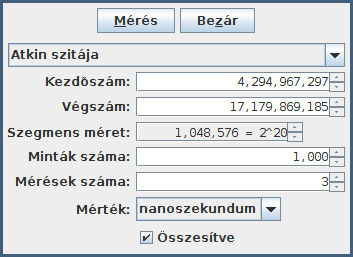
\includegraphics[scale=1.0]{measure.png}
\end{figure}

A sziták listája ugyanaz, mint a sziták ellenőrzősénél.
A mintákat a program a szitált intervallumon egyenletesen osztja el a megadott méretű szegmensek határainál.
A teljes szitálást annyiszor végzi el, amennyi a mérések számában meg volt adva, és az eredményt átlagolja.
Összesítést kiválasztva a mintaelemek értéke a szitált intervallum elejétől az adott számig szitálás teljes ideje, különben az előző minta helyétől.
A mérték szabályozza, hogy a tényleges eltelt időt mérje a program nanoszekundumokban, vagy az elvégzett műveletek számát.

\subsection{Minta közelítése}

Az ablak jobb oldalának középső harmadában a kiválasztott minta részletei látszódnak.
Itt változtatható meg a minta ábrázolásához használt szín, távolítható el a minta, vagy menthető CSV fájlba.

A táblázat a minta közelítéseit mutatja, itt olvashatóak le a közelítés komponensfüggvényei, és a közelítés hibája.
A ''Közelítés'' gombbal lehet új közelítést hozzáadni az ábrázoláshoz.
A közelítéshez a lineáris legkisebb négyzetek módszerét használja a program, ehhez a lineáris kombináció elemi függvényeit meg kell adni.
A függvények kiválaszthatóak az előre megadott listából, vagy JavaScript nyelven is megadhatóak.
A közelítéshez csak olyan függvények használhatóak, amik a minta minden pontjában értelmezve vannak.

\begin{figure}[H]
\caption{A közelítés elemi függvényeinek megadása}
\centering
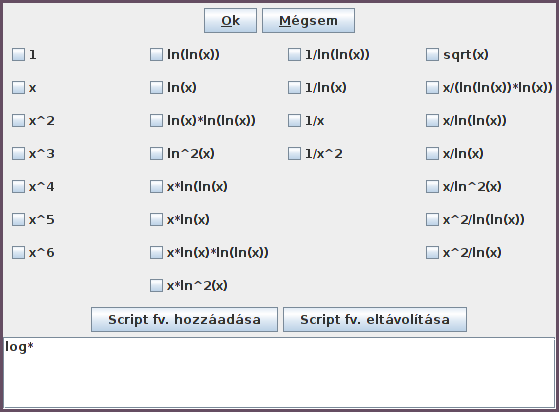
\includegraphics[scale=0.75]{functions}
\end{figure}

JavaScript függvényhez meg kell adni a függvény nevét és forráskódját.
A forráskódban a függvény argumentumára az $x$ változóval lehet hivatkozni, és a szkript utolsó kifejezésének értéke lesz a függvény értéke $x$-ben.
Pl. az $x \mapsto \frac{\ln{x}}{x}$ hozzárendelés forráskódja:

\begin{lstlisting}[basicstyle=\small, language=Java]
Math.log(x)/x
\end{lstlisting}

A szkriptben használható változó, és a szokásos vezérlőutasítások.
Pl. az iterált logaritmus egy megadása:
\begin{lstlisting}[basicstyle=\small, language=Java,morekeywords=var]
var y=0;
while (1<x) {
  x=Math.log(x);
  ++y;
}
y
\end{lstlisting}

Az így megadott függvények visszatérési értéke mindig \texttt{double} típusú kell legyen,
és a függvény azokban a pontokban értelmezett, ahol ez az érték véges.

Egy kiválasztott közelítés részletei az ablak jobb alsó sarkában látszódnak, itt megváltoztatható a közelítéshez rendelt szín, és eltávolítható a közelítés.
A táblázat a közelítéshez kiválasztott függvények együtthatóit mutatja a lineáris kombinációban.

A legkisebb négyzetek módszerének feladata röviden leírható.
Ha az $n$ elemű minta
\begin{align*}
(x_1, y_1), (x_2, y_2), \ldots, (x_n, y_n) (x_i \in \mathbb{N}, y_i \in \mathbb{R})
\end{align*}
és a közelítéshez kiválasztott $m$ függvény
\begin{align*}
f_1, f_2, ..., f_m (f_i:\mathbb{R} \mapsto \mathbb{R})
\end{align*}
akkor a legkisebb négyzetek módszere keresi azokat a
\begin{align*}
c_1, c_2, ..., c_m (c_i \in \mathbb{R})
\end{align*}
skalárokat, hogy az
\begin{align*}
f(x)=\sum_{i=1}^m c_i f_i(x) (x \in \mathbb{R})
\end{align*}
közelítő függvény és a minta eltérése minimális
legyen a
\begin{align*}
\sum_{i=1}^{n} (f(x_i)-y_i)^2
\end{align*}
négyzetes eltérés összeg szerint.

A program ezt az eltérés összeget jeleníti meg a közelítés hibájaként, valamint a $c_i$ skalárok a közelítés elemi függvényeinek együtthatói.

\section{Sziták mérése szkriptekkel}

A sziták futási idejének mintáit parancssorból is elő lehet állítani.
Ilyenkor az eredményt, megjelenítés helyett, a megadott fájlba írja a \texttt{gui} program, ami később a grafikus felületen betölthető.
A méréseket a \texttt{measure-sieve} szkripttel lehet elvégezni, paraméterként meg kell adni ebben a sorrendben:
\begin{itemize}
\item a szita nevét, ezek ugyan azok lehetnek, mint a \pageref{sec:szitak-ellenorzese} oldalon a ''Sziták ellenőrzése'' szakaszban
\item a számot, ahol a szitálás kezdődik, ez páratlan szám kell legyen
\item a szitálás végét, ez páratlan szám kell legyen
\item a szegmensek méretét
\item a mérések számát
\item a minták számát
\item hogy időt (\texttt{nanosecs}), vagy műveleteket (\texttt{operations}) mérjen
\item összesítse az időket (\texttt{sum}), vagy szegmensenként külön számolja (\texttt{segment})
\item a fájlt, ahova az eredményt mentse CSV-ben
\end{itemize}

Ha a kezdőszám nagyobb, mint 1, akkor az adatbáziskönyvtárnak tartalmaznia kell az \texttt{init} program generálta első négy szegmenst.

Lehetőség van a mérték és az összesítés mind a négy kombinációját egy méréssel előállítani, ehhez mind a négy kimeneti fájl meg kell adni külön.

\begin{lstlisting}[language=bash]
scripts$ ./measure-sieve buckets-3 1 0x10000001 0x10000 3 1000 nanosecs sum out1.csv
100.0%
scripts$ ./measure-sieve buckets-3 1 0x10000001 0x10000 3 1000 operations segment out2.csv
100.0%
scripts$ ./measure-sieve buckets-3 1 0x10000001 0x10000 3 1000
seg-ns.csv seg-ops.csv sum-ns.csv sum-ops.csv
100.0%
\end{lstlisting}

A mérések megkönnyítéséhez a \texttt{measure-sieves} szkript az összes szitát megméri, és az eredményt a \texttt{samples} könyvtárba menti.
A \texttt{samples} könyvtárban a mérési eredmények 4 külön könyvtárban szegmensenként/összesítve, és idő/művelet szerinti bontásban vannak.
Ezekben a könyvtárakban 2 fajta mérés eredményei vannak.
Az \texttt{atkin} könyvtárban Atkin szitájának sebessége van megmérve különböző szegmensméretek esetén.
Azokban könyvtárakban, amiknek a neve \texttt{speed}-del kezdődik, az összes szita sebességének mérése található, $2^{20}$ szegmensmérettel.
A könyvtárak nevében a szám a szitálás kezdetét adja meg, a \texttt{speed}$n$ nevű könyvtárban a mérések $2^n+1$-től kezdődnek.
A lassabb szitákat csak kisebb nagyságrendekre méri meg a szkript, ezek futási ideje hamar túl naggyá válik.

A \texttt{measure-generator} szkript a \texttt{generator} program sebességét méri meg.
A mérés 3 paramétert variál, a szitálás kezdetének nagyságrendjét, a szegmensméretet, és az edénysor számrendszerét.
Az eredményt a \texttt{samples/measure-generator.csv} fájlba menti.
Ez nem használható a program mintamegjelenítésével, mert az egy változós mintákkal dolgozik.
Ennek a mérésnek a célja az, hogy a \texttt{generator} program paramétereit egy konkrét számítógéphez lehessen igazítani.
A szkript 16 egymás utáni szegmensfájlt szitál,
\begin{itemize}
\item a szitálás kezdetét $2^{33}$-től $2^{63}$-ig változtatja, a kitevőt hármasával növelve
\item a szegmensek méretét $2^{16}$-tól $2^{24}$-ig, a kitevőt egyesével növelve
\item és a számrendszert $2^1$-től $2^8$-ig, szintén a kitevőt egyesével növelve.
\end{itemize}

%%% Local Variables:
%%% mode: latex
%%% TeX-master: "szakdolgozat"
%%% End:
